\documentclass[a4paper]{report}

\usepackage{amsmath, siunitx, titlesec, hyperref}
\usepackage[dutch]{babel}
\usepackage[official]{eurosym}
\usepackage{graphicx}
\graphicspath{{./img/}}
\usepackage{tikz}
\usetikzlibrary{shapes.geometric, arrows}
\tikzstyle{object} = [rectangle, minimum width=3cm, minimum height=1cm, text centered, draw=black]
\tikzstyle{arrow} = [thick]

\definecolor{light-gray}{gray}{0.95}
\newcommand{\code}[1]{\colorbox{light-gray}{\texttt{#1}}}

%Reformat title
\titleformat{\chapter}
  {\normalfont\LARGE\bfseries}{\thechapter}{1em}{}
\titlespacing*{\chapter}{0pt}{3.5ex plus 1ex minus .2ex}{2.3ex plus .2ex}

\title{Rapport projectwerk 1\\ Biometrisch station}
\author{Jonas Meeuws \and Jonas Van Dycke}
\date{Academiejaar 2017-2018}

\begin{document}

\maketitle
\tableofcontents

\chapter{Voorwoord}

\chapter{Omschrijving}
    \section{Doelstellingen}
        Het doel van dit project is om gegevens uit sensoren te halen en ze te visualiseren.
        Er worden gegevens gegenereerd door verschillende sensoren die verbonden zijn aan een Arduino.
        De Arduino hangt aan de USB-poort van een computer.
        Er draait een java daemon op die computer die communiceert met de Arduino.
        De daemon zendt de gegevens via Mqtt naar een andere computer waar een grafisch javafx-programma op draait.
        Het grafisch programma visualiseert de gegevens van meerdere stations aan de hand van grafieken.

    \section{Blokschema}
        %JM
        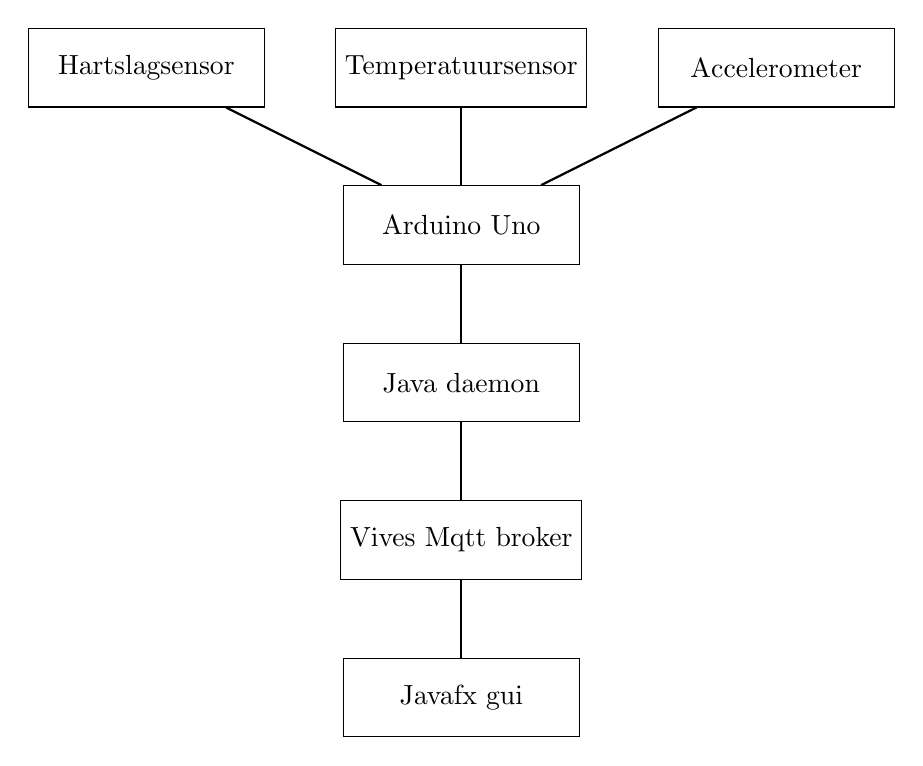
\begin{tikzpicture}[node distance=2cm]
            \node (arduino) [object] {Arduino Uno};
            \node (temp) [object, above of=arduino] {Temperatuursensor};
            \node (heart) [object, left of=temp, xshift=-2cm] {Hartslagsensor};
            \node (accel) [object, right of=temp, xshift=2cm] {Accelerometer};
            \node (daemon) [object, below of=arduino] {Java daemon};
            \node (broker) [object, below of=daemon] {Vives Mqtt broker};
            \node (gui) [object, below of=broker] {Javafx gui};
            \draw [arrow] (temp) -- (arduino);
            \draw [arrow] (heart) -- (arduino);
            \draw [arrow] (accel) -- (arduino);
            \draw [arrow] (arduino) -- (daemon);
            \draw [arrow] (daemon) -- (broker);
            \draw [arrow] (broker) -- (gui);
        \end{tikzpicture}
        
    \section{Schakeling}
        %JVD
        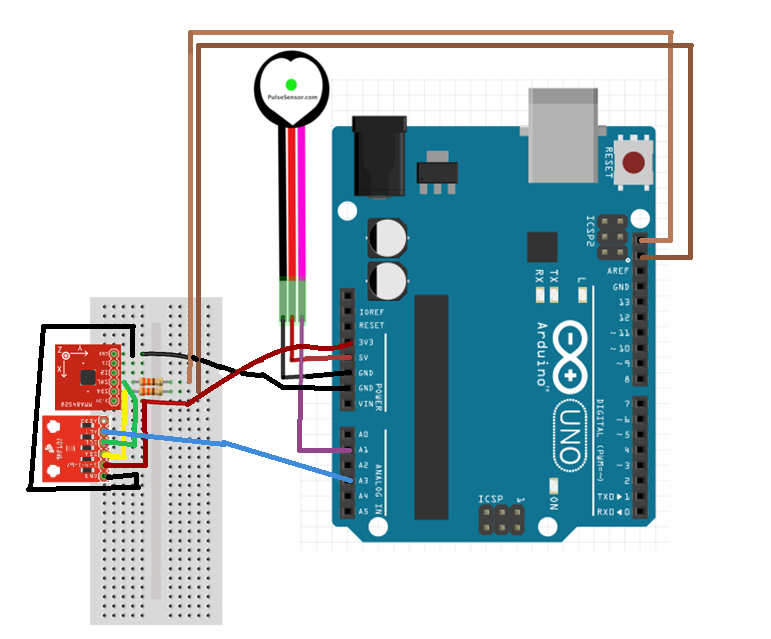
\includegraphics[width=\textwidth]{schema}\\
        Op de arduino zijn er 3 sensoren (Temperatuursensor, Accelerometer en Hartslagsensor) aan gekoppeld om de waarden van de sensoren te kunnen meten.
        Hierbij worden de waarden van de sensoren zichtbaar wanneer er op de knoppen van de "LCD BUTTON SHIELD V2" word gedrukt.
        Daarom bij het opstarten van de arduino komt er op de LCD scherm te voorschijn welke knop ingedrukt moet worden voor de sensor waarden te kunnen zien.
        De gemeten waarden worden van de arduino naar de "Vives Mqtt broker" gestuurd, om zo via "Javafx gui" een grafiek kunnen voorstellen van deze gemeten waarden.
    
\chapter{Planning}
    \section{Taakverdeling}
        %JM
        Jonas Meeuws heeft beide Java applicaties volledig geschreven en een deel van de Arduino software (serial).
        Jonas Van Dycke heeft de schakeling gemaakt en deels de Arduino software geschreven.
        Tijdens de labo's werkten we vooral samen aan de Arduino software.\\
        De inhoud van dit verslag werd door ons beide geschreven (zie commentaar).
        Het document werd opgesteld door Jonas Meeuws.
        
    \section{Git}
        %JM
        Voer \code{git blame} uit in de mappen van de gezamelijke delen om lijn per lijn te zien wie welk stuk geschreven heeft.
        De commits van de Arduino software en het verslag tijdens de lesuren zijn samen gemaakt.
        Jonas Van Dycke is ``unknown''.
        Gebruik \code{git log} om revisions te zien en \code{git checkout [revision id]} om naar een vorige versie te gaan.
        Gebruik \code{git checkout master} om naar de laatste versie te gaan.
        
\chapter{Hardware}
    \section{Eagle schema}
        %JVD
        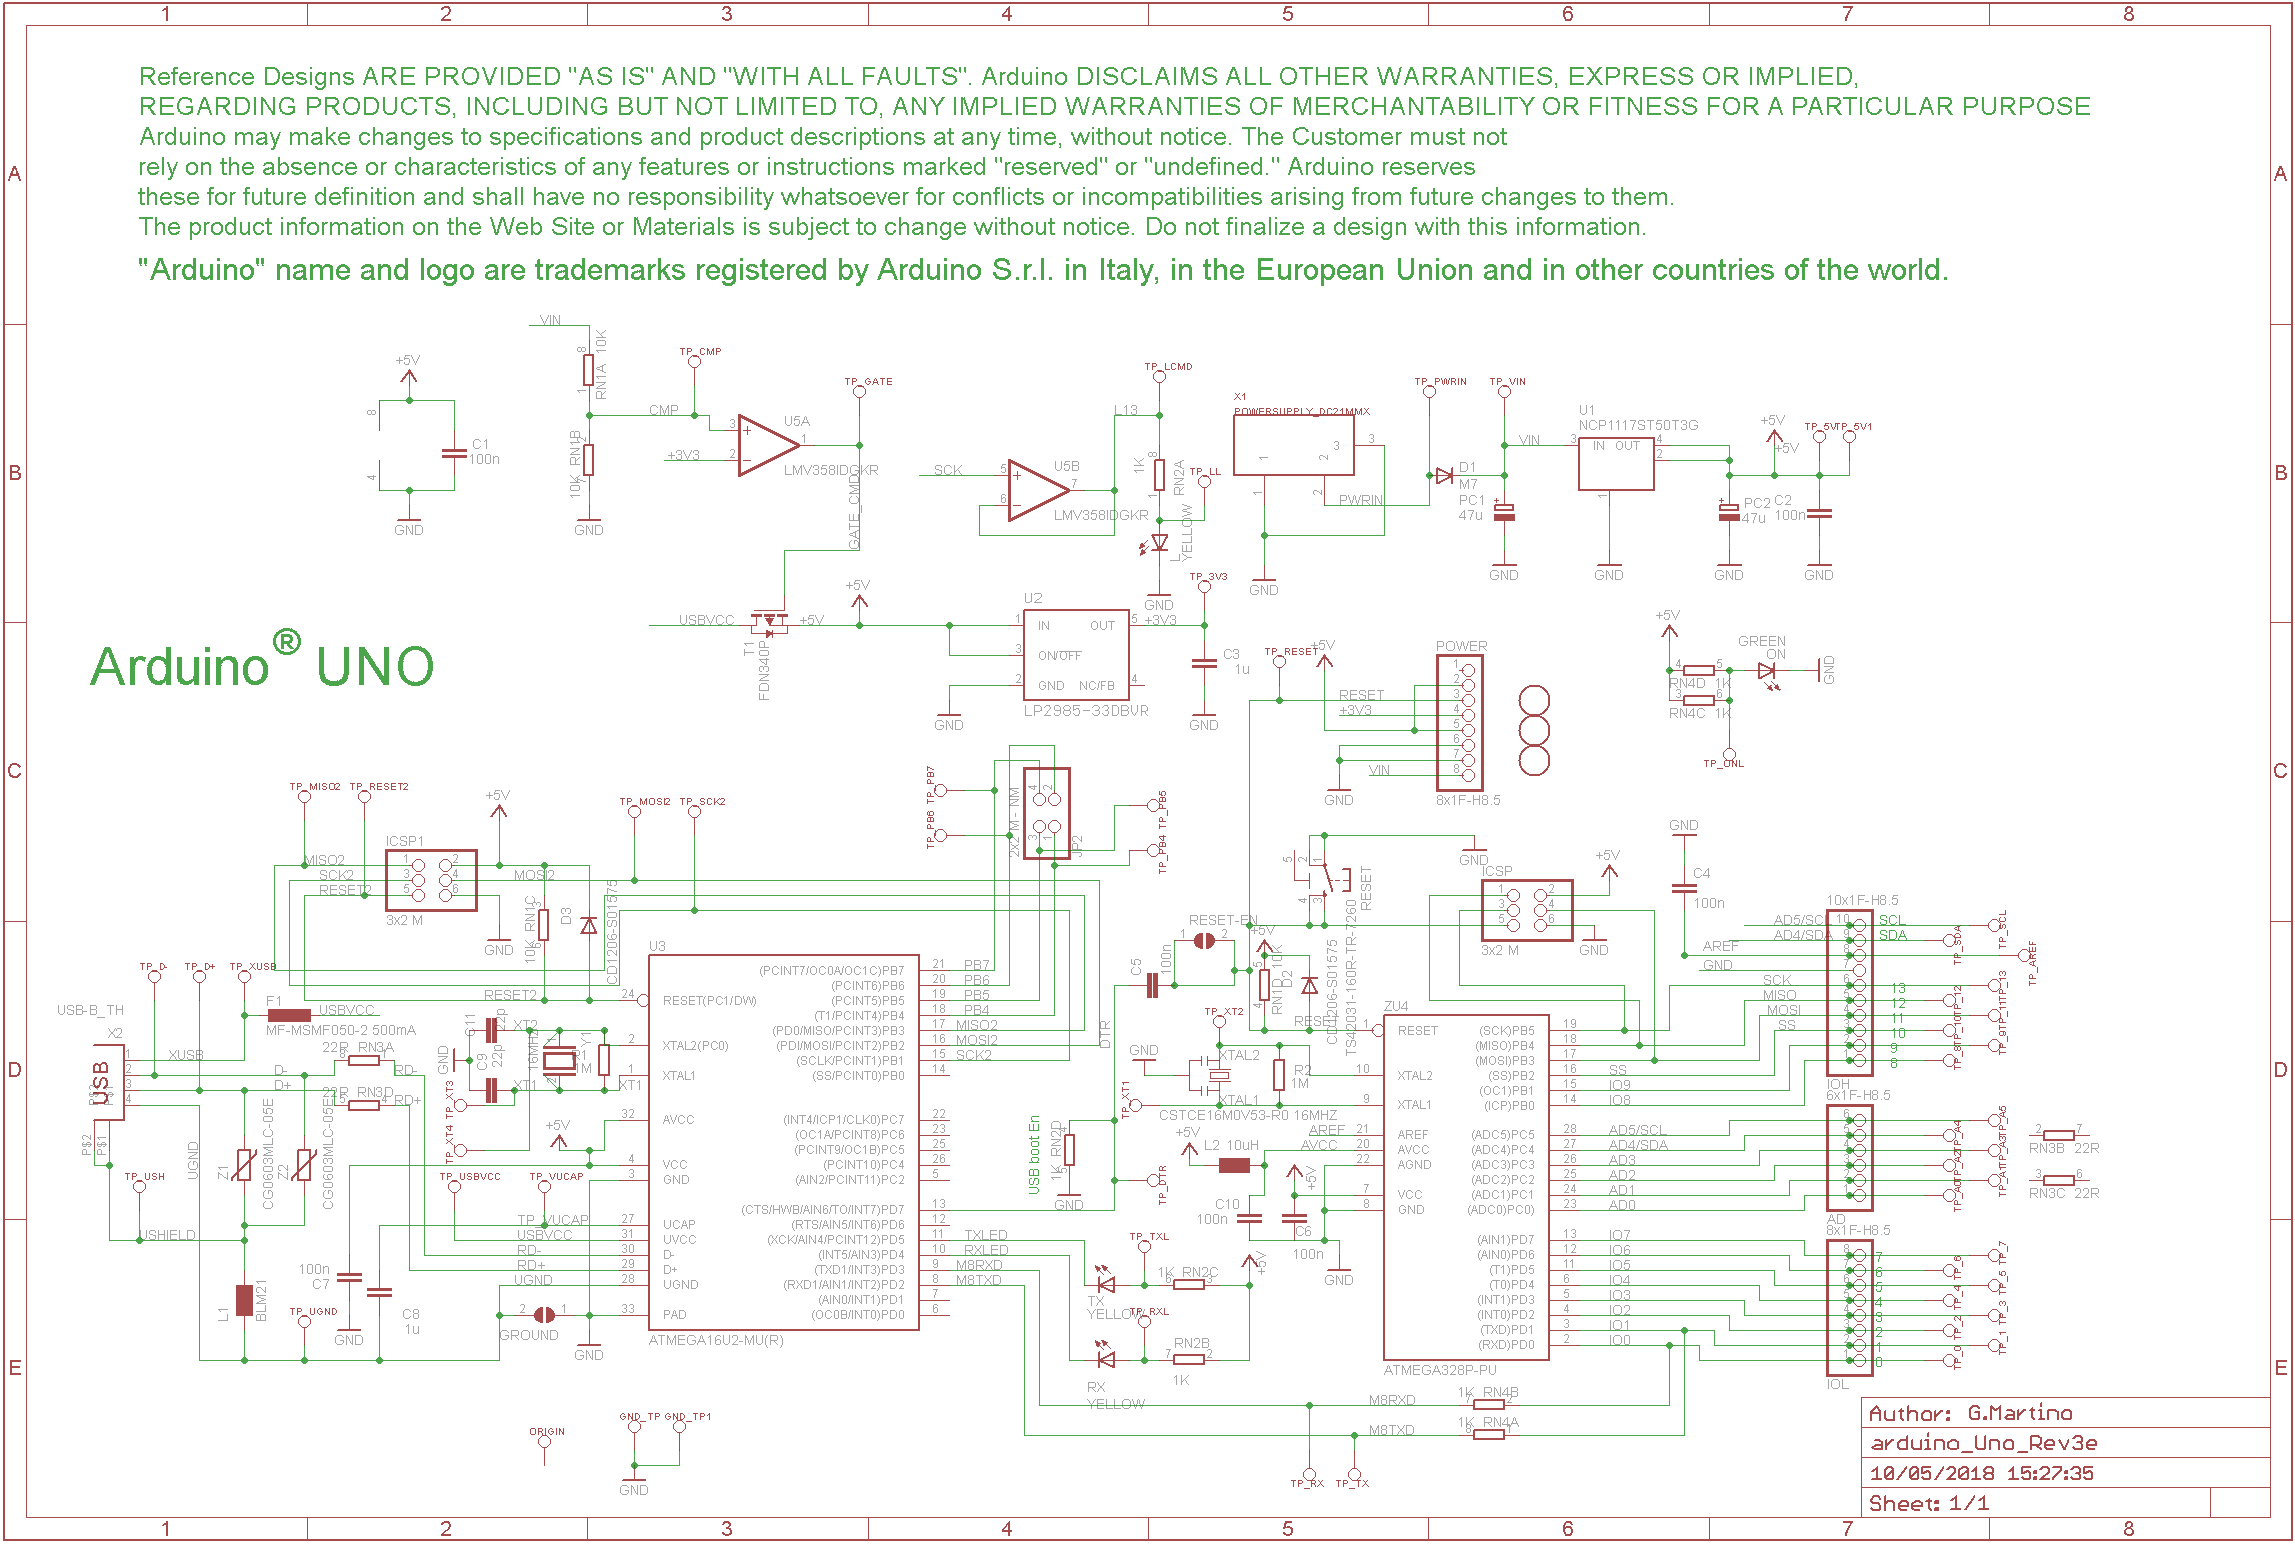
\includegraphics[width=\textwidth]{ArduinoUno_Schema}
        %"16X2_LCD_shield.pdf"
        
    \section{Eagle board}
        %JVD
        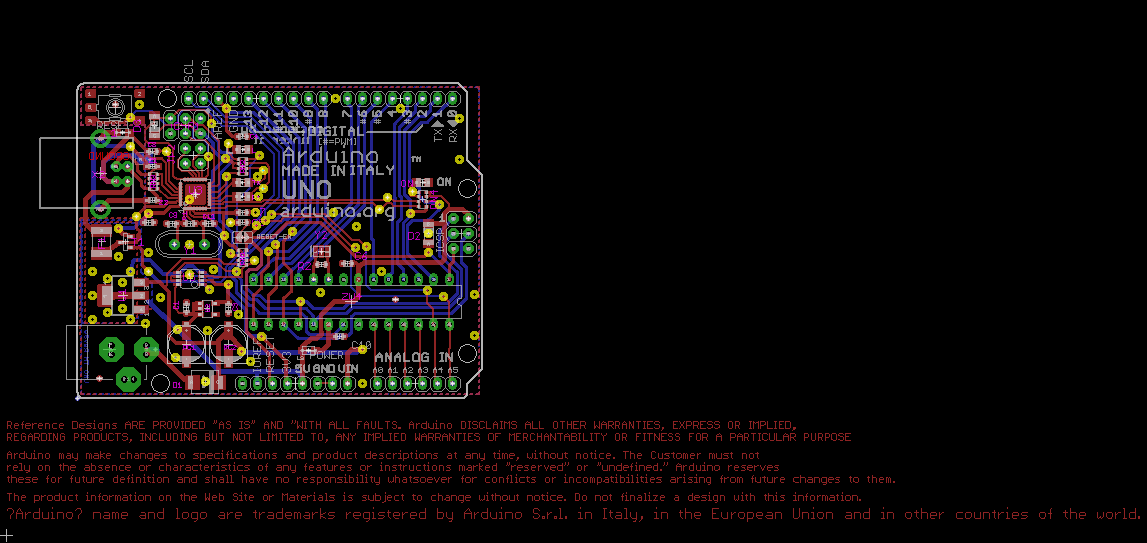
\includegraphics[width=\textwidth]{ArduinoUno_Board}
        %"16X2_LCD_shield.pdf"
        
    \section{Stuklijst (BOM = Bill of Materials)}
        %JVD
        \begin{tabular}{|c|c|}
            \hline
            Component & Prijs\\
            \hline
            Arduino UNO                        & \euro $20.00$\\
            Pulse Sensor                       & \euro $24.95$\\
            TEMPERATURE SENSOR                 & \euro $4.95$\\
            LCD BUTTON SHIELD V2               & \euro $12.95$\\
            Triple Axis Accelerometer Breakout & \euro $8.46$\\
            \hline
        \end{tabular}
        
    \section{Kostprijsberekening}
        %JVD
        \begin{tabular}{|c|c|}
            \hline
            Totale kost prijs & \euro $61.31$\\
            \hline
        \end{tabular}
        
    \section{Overzicht connectoren}
        %JVD
    2xWeerstanden ($330\si\ohm$)
    
    \section{Overzicht test-pinnen}
        %JVD

    \section{Stuklijst (BOM = Bill of Materials)}
        %JVD
    
        \subsection{Component: heart pulse sensor amped}
            \begin{tabular}{|c|c|}
                \hline
                Draden & Pin\\
                \hline
                rood  & J1 Nr:3 (5V)\\
                zwart & J1 Nr:5 (GND)\\
                paars & J2 Nr:2 (A1)\\
                \hline
            \end{tabular}

        \subsection{Component: Accelerometer (MMA8452)}
            \begin{tabular}{|c|c|}
                \hline
                Pin component & Pin Arduino\\
                \hline
                3.3V & J1 Nr:2 (3.3V)\\
                SDA  & SDA\\
                SCL  & SCL\\
                I2   & /\\
                I1   & /\\
                GND  & J1 Nr:4 (GND)\\
                \hline
            \end{tabular}
            
        \subsection{Component: Temperature meter (TMP102)}
            \begin{tabular}{|c|c|}
                \hline
                Pin component & Pin Arduino\\
                \hline
                GND  & J1 Nr:4  (GND)\\
                3.3V & J1 Nr:2  (3.3V)\\
                SDA  & SDA\\
                SCL  & SCL\\
                ALT  & J2 Nr:4  (A3)\\
                ADD0 & /\\
                \hline
            \end{tabular}
            
    \section{Digitale foto’s van opstellingen}
        %JVD
        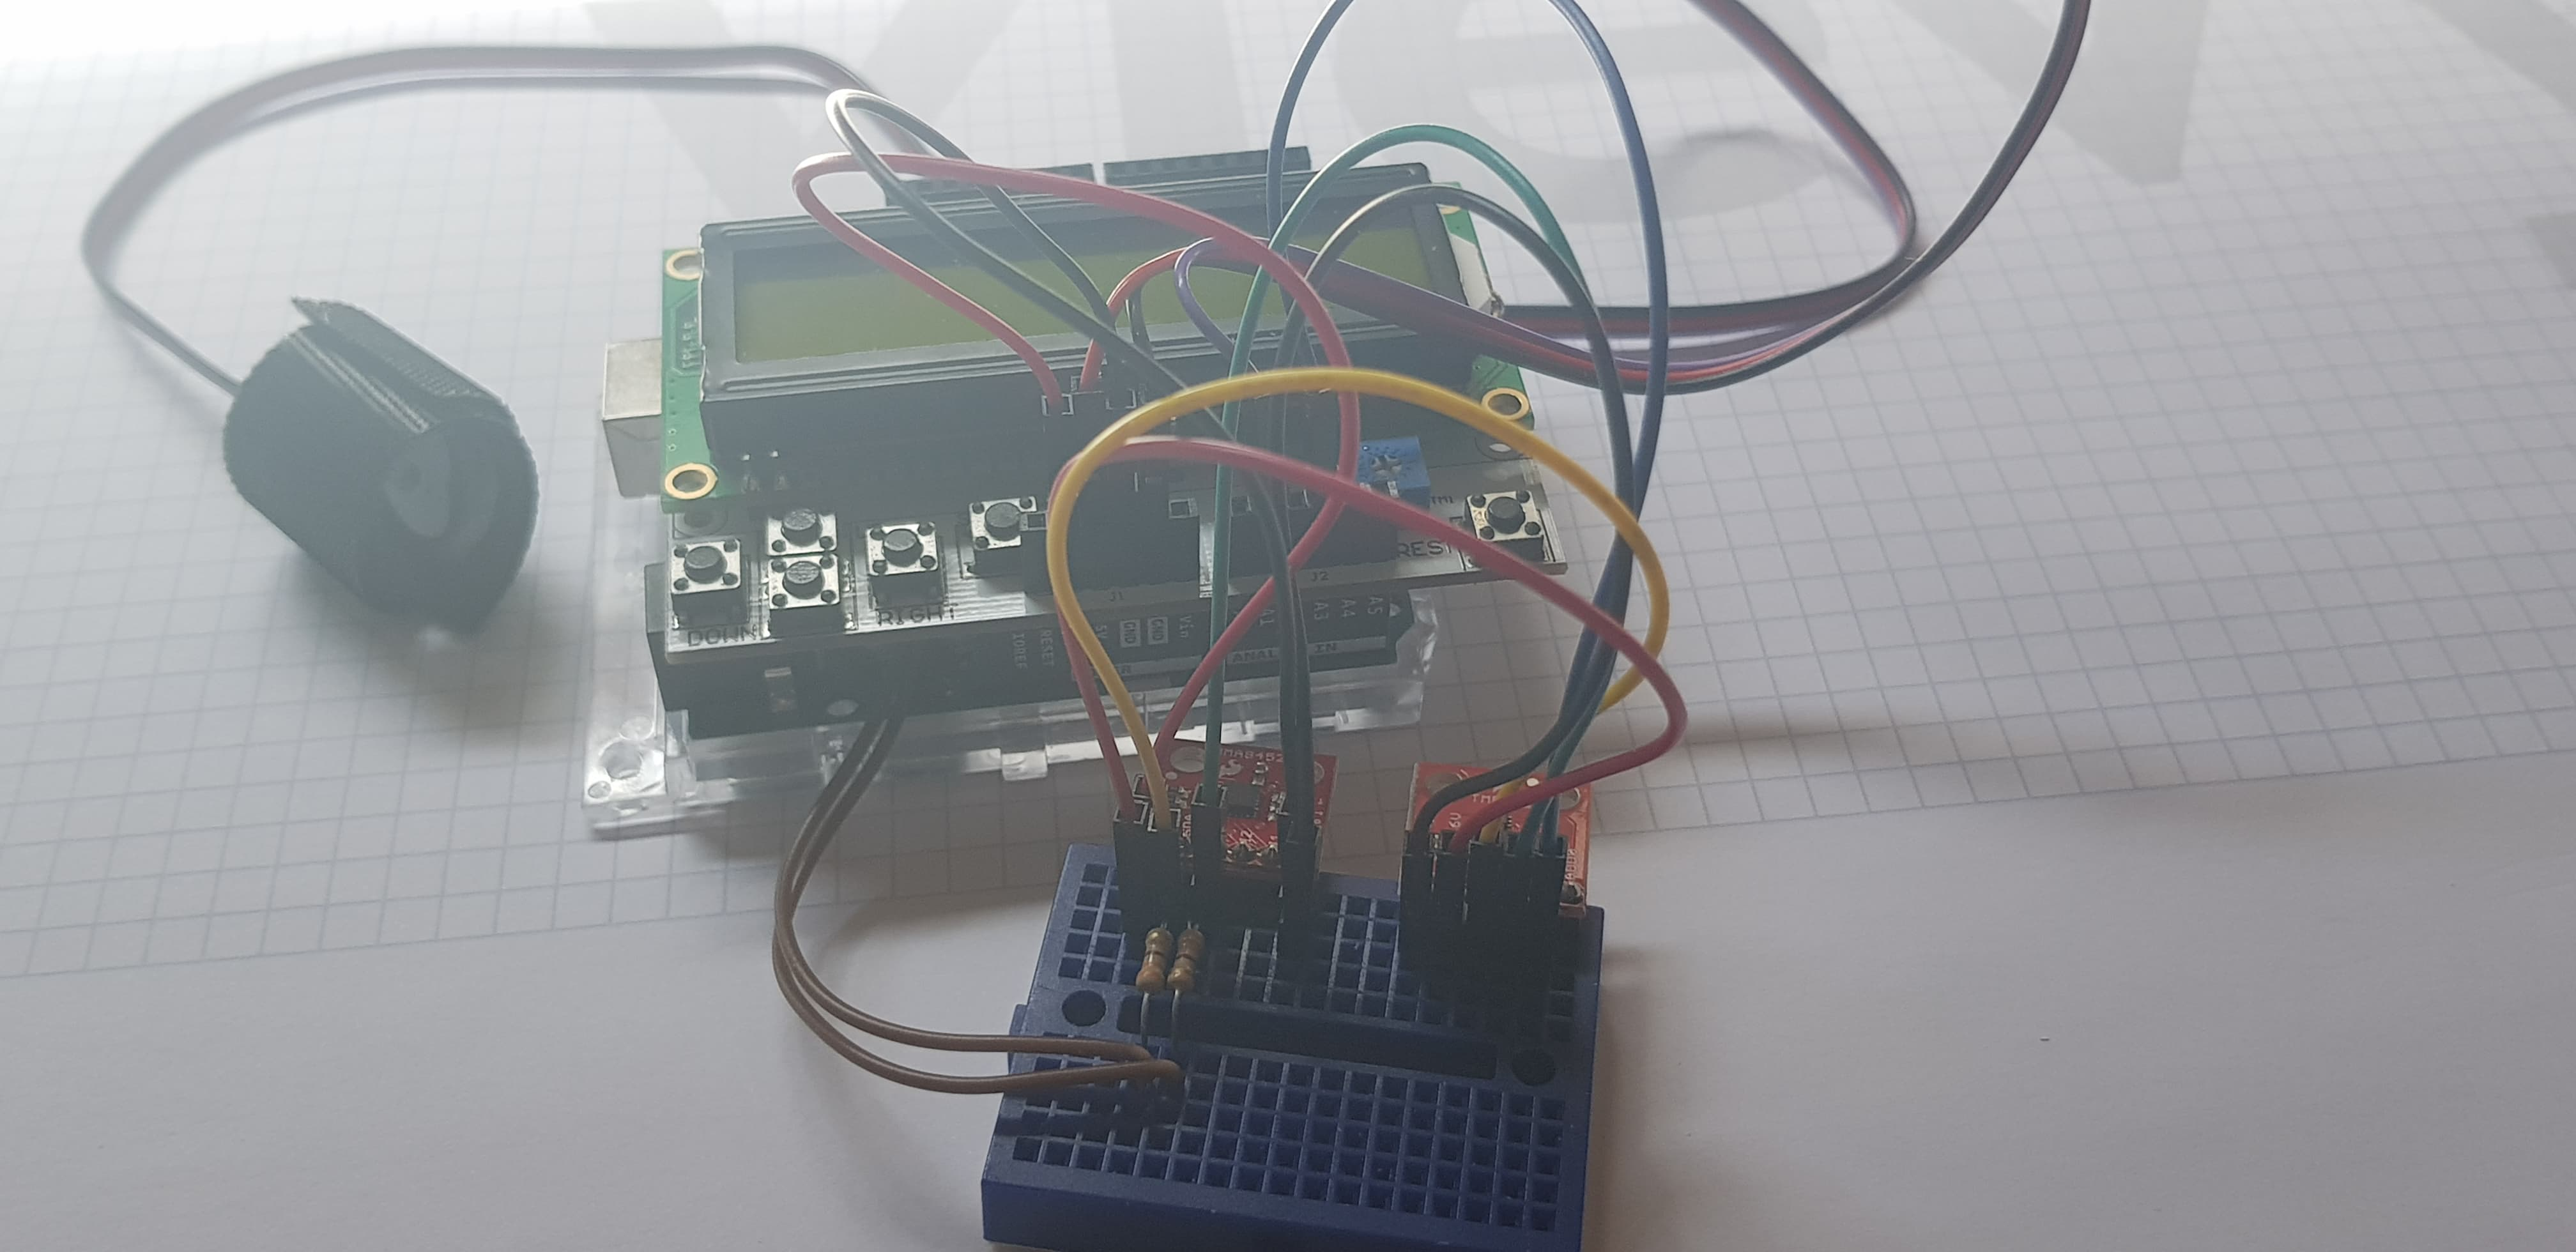
\includegraphics[width=\textwidth]{Fysieke_Voorstelling1}\\
        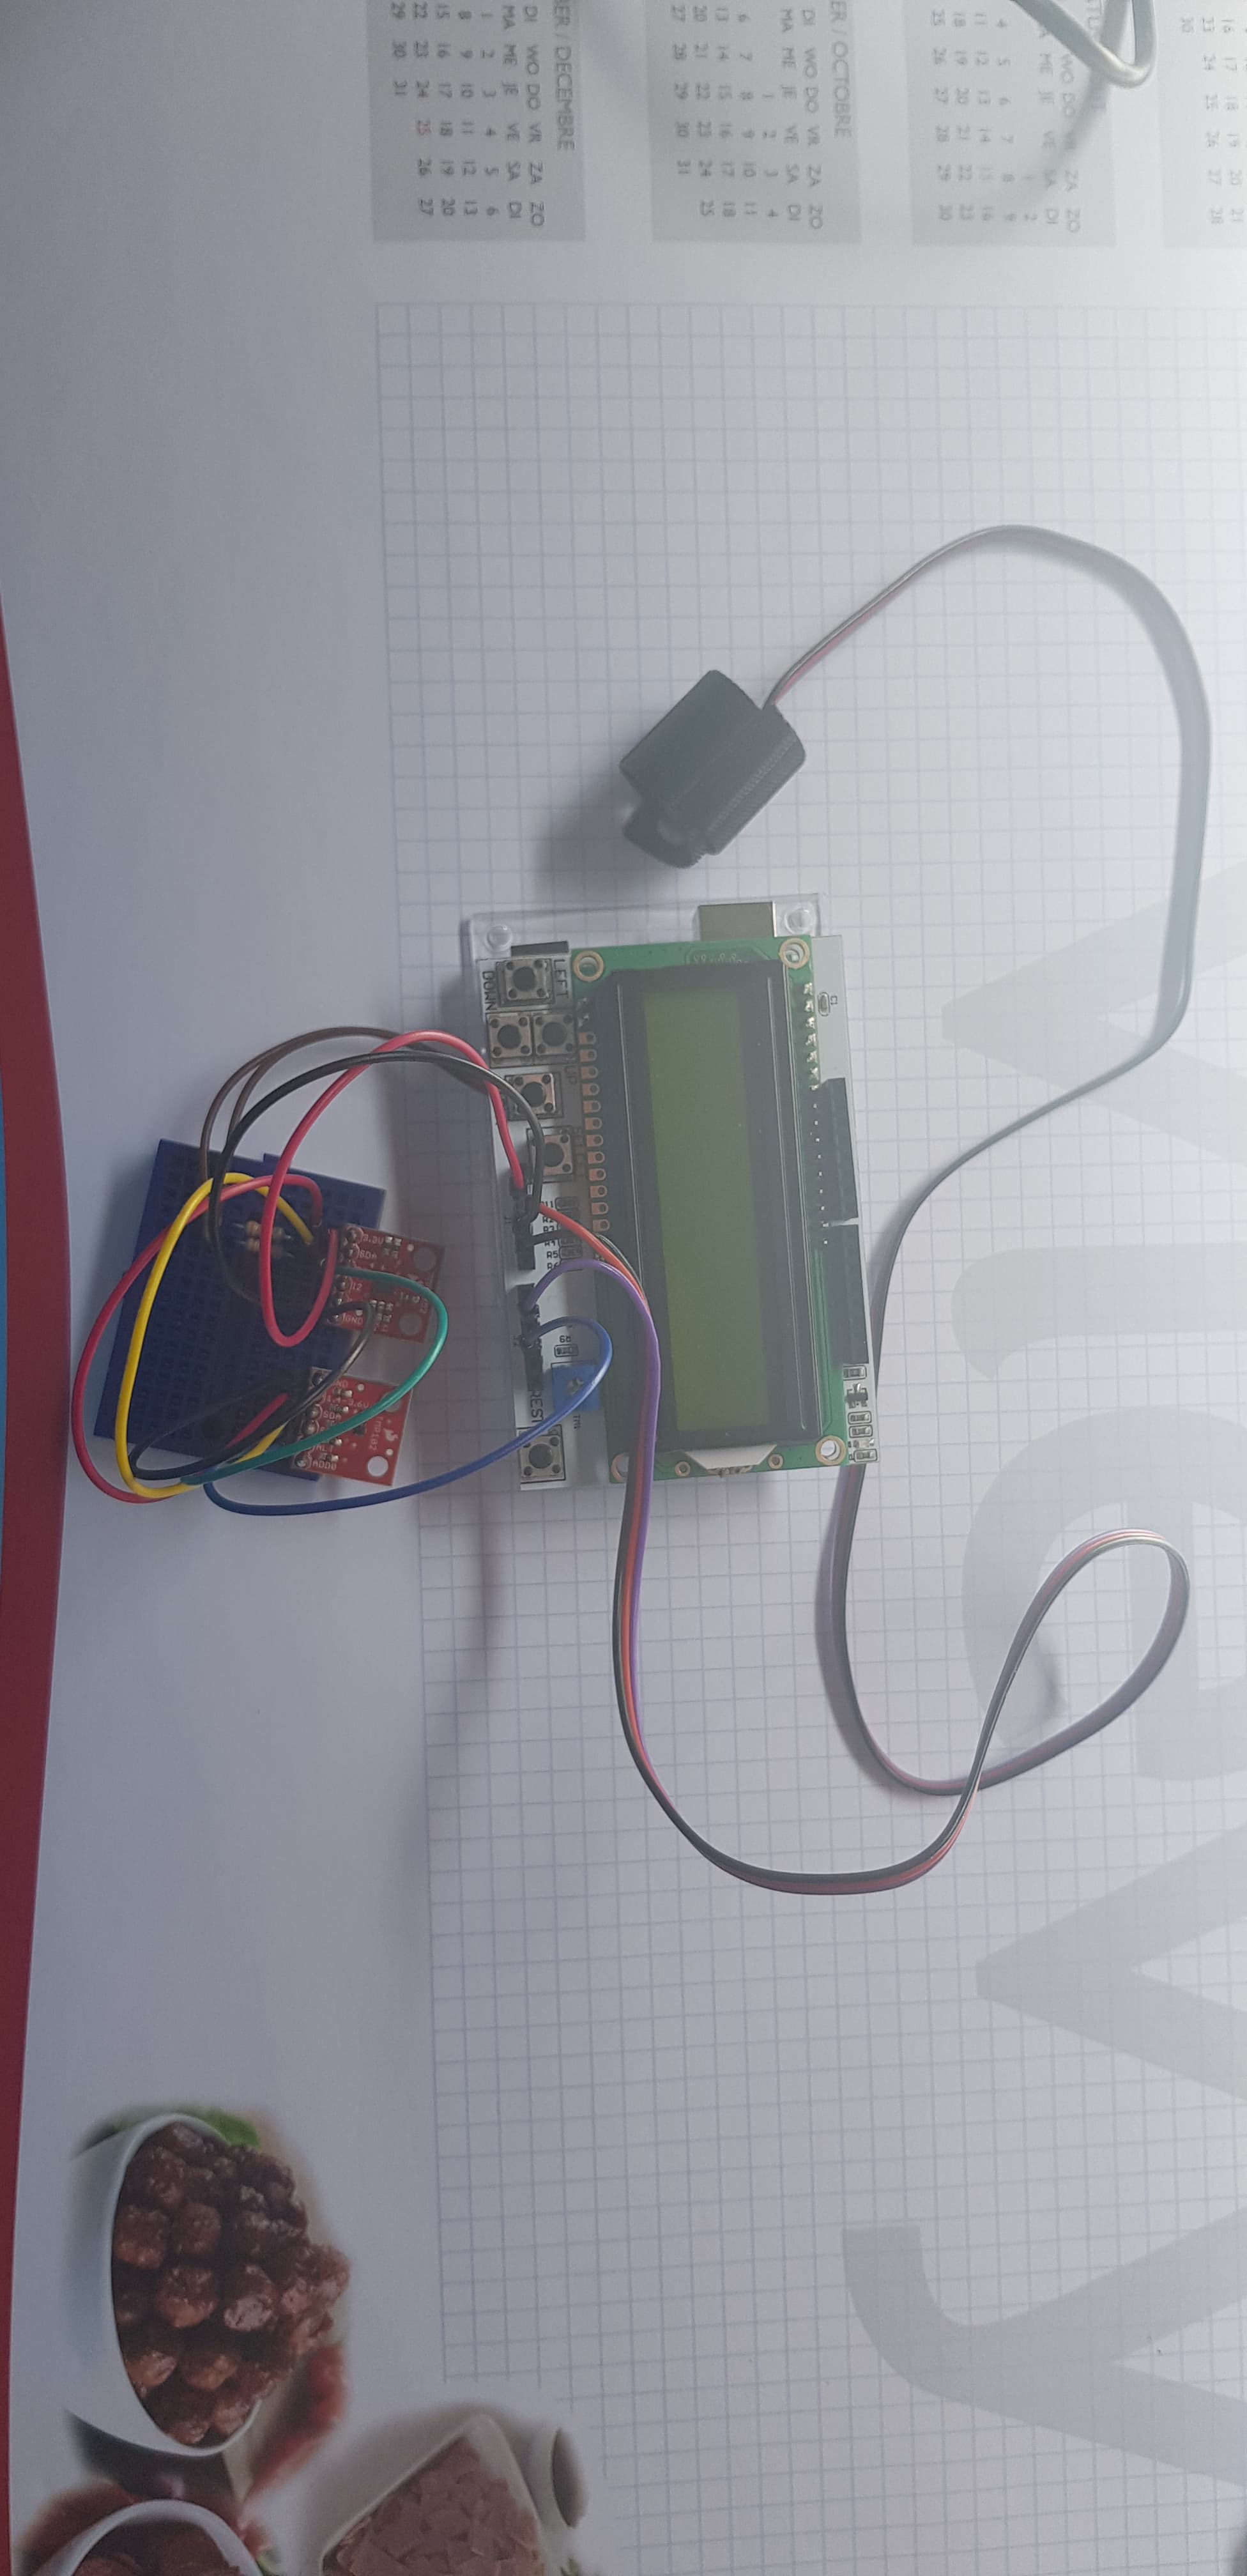
\includegraphics[width=\textwidth]{Fysieke_Voorstelling2}
    
\chapter{Software}
    \section{Arduino}
        \subsection{Main}
            %JVD
            De code van de arduino bestaat uit 7 verschillende tabbladen, die zelf verschillende classes bevatten
            (main, Accelerometer, Button, HeartRate, Lcd, SerialController,Temperature).
            \subsection{De main}
                In de main komen alle codes samen, om zo de gewenste eind resultaat te bekomen.
                
            \subsection{De Accelerometer}
                Hierin worden de waarden die gemeten worden door de MMA8452 \cite{accel5} via de poort SDA naar de arduino gebracht.
                De arduino zet deze data om naar X, Y en Z waarvan de waarden visueel op de LCD kunnen zien.
                Om dit te kunnen doen werken moeten de gevraagde 'library' toegevoegd worden.
                
            \subsection{De HeartRate}
                Hierbij komt er via Pin A1 een analoge spanning toe die door de pulssensor gemeten word, om zo de hardslag te kunnen meten.
                Om de digitale waardes te kunnen krijgen voor de LCD moet de gemeten waarden op A1 laten lezen in 'analogRead'.
                
            \subsection{De Temperature}
                We meten de waarden van de temperature aan de hand van pin A3.
                Hier worden de gemeten waarden omgezet in °C, om zo de waarde op de LCD te kunnen plaatsen.
                Om dit te kunnen doen werken moeten de gevraagde 'library' toegevoegd worden.
                
            \subsection{De LCD}
                Hier in worden de texten met de gemeten waarden samen gevoegd om zo duidelijk de waarden via de LCD te kunnen lezen.
                Om de LCD te kunnen doen werken moet er eerst de 'library' van de LCD weergeven met de pinnen waar de LCD verbonden mee is.
                Als de verbonden pinnen niet weergeven is, dan zal de LCD ook niet werken.
                We beschrijven de in deze code de HeartRate, Temperature en de Accelerometer samen met de gemeten waarden.
                
            \subsection{Button}
                In deze code beschrijven we welke gemeten waarden te voorschijn komt bij het drukken van de knoppen (left, right en down).
                We beschrijven welke knop ingedrukt word door elke knop tussen een bepaalde waarde te steken.
                Deze waarden worden analoog gelezen en omgezet, om zo de drukknoppen doen werken.
                (PS individueel werken de knoppen, maar bij het samen steken van de codes zijn de waarden verandert waardoor de knoppen niet meer werken).
                
            \subsection{SerialController}
                Bij deze code worden alle waarden die gemeten worden mooi bij elkaar geplaatst.
                
    \section{Java parser daemon}
        %JM
        Het doel van de parser is om waarden uit de Arduino te krijgen over de seri\"ele poort en ze via Mqtt te verzenden.

        \subsection{Main}
            De Main classe maakt een nieuw object van \code{BiometricsParser} aan en roept zijn constructor aan.

        \subsection{BiometricsParser}
            De constructor roept eerst \code{initialize()} aan.
            Het programma wacht tot er een Arduino aangesloten wordt en stelt de baud rate van de poort in op $115200$ Bd.
            Hierna begint de ``main loop''. Het programma wacht tot de \code{SerialPort} data beschikbaar heeft.
            De data wordt uitgelezen door \code{readMessage()} en wordt opgeslagen in een variabele.
            Daarna wordt er een \code{BiometricsData} object samengesteld met behulp van de parser.
            In \code{SendMessage()} wordt er met Gson een json-string gemaakt van het \code{BiometricsData} object.
            Ten slotte wordt deze string met de MqttService verzonden naar de Mqtt broker, waarna de loop opnieuw begint.
            Wanneer de Arduino wordt losgekoppeld, wordt het programma afgesloten.

        \subsection{Parser} 
            De statische methode \code{Parser.parse()} kan gebruikt worden om een \linebreak\code{BiometricsData} object te maken van een string.
            Intern wordt er een methode \code{isValid()} gebruikt om te controleren of de string wel aan het protocol voldoet.
            Als dit niet het geval is, wordt het bericht weggesmeten.
            Het bericht wordt omgezet in een array van doubles door te zoeken naar de locaties van de separators.
            De methode \code{Double.parseDouble()} wordt gebruikt om strings in doubles om te zetten.
            De methode \code{parse()} maakt een nieuw \code{Biometricsdata} object met alle waarden en de naam van het station in.
            Dat object wordt meegegeven als de return value.

        \subsection{BiometricsData}
        \label{sec:biometricdata}
            \code{BiometricsData} is een classe die zowel bij de daemon als de grafische applicatie gelijk is.
            Dit is omdat ze aan de hand van Gson wordt gebruikt als communicatieprotocol.
            De classe heeft een naam en 3 waarden als attributen, een constructor en enkele getters en setters.
            De waarde \code{acceleration} is een object van de classe \code{Acceleration}, wat \code{BiometricsData} een compound maakt.
            De classe \code{Acceleration} bestaat uit een x-, een y- en een z-acceleration als attributen, met een paar getters en setters.

        \subsection{MqttService}
        \label{sec:mqttservice}
            Deze classe komt uit een andere opdracht, de ``Chat client''.
            In de \linebreak\code{BiometricsParser} wordt er een object gemaakt van deze classe.
            Hierna kan \code{sendMessage()} gebruikt worden om een bericht te verzenden op de topic \code{biometrics/general}.
            Behalve de naam van de base topic is er niets veranderd aan de classe.

    \section{JavaFX visualisatie}
        %JM
        \subsection{BiometricsGuiController}
            Dit is de ``M̀ain'' classe van de gui.
            De attributen bestaan uit 4 fxml-objecten, de grafieken.
            Een \code{ArrayList} houdt de stations bij en een index houdt de huidige x-waarde bij.
            Nadat de grafische omgeving is aangemaakt, wordt \code{initialize()} aangeroepen.
            De \code{ChatService} wordt ingesteld en de \code{SeriesManager} wordt aangemaakt.
            De \code{ChatService} zorgt ervoor dat we een methode \code{MessageArrived()} kunnen maken volgens een interface.
            Wanneer er een bericht binnenkomt, wordt \code{MessageArrived()} aangeroepen met als argumenten het channel en het bericht.
            Met behulp van de Gson-library kunnen we van het bericht een nieuw object van \code{BiometricData} maken.
            Als de naam van het station nog niet voorkwam wordt er een nieuw station gemaakt.
            Nadat het station bestaat, wordt zijn object opgezocht in de \code{ArrayList} door \code{getStation()}.
            Ten slotte wordt de data aan de grafieken toegevoegd.
            
        \subsection{Station}
            Elk object van \code{Station} definieert een apart station.
            Wanneer de contructor wordt aangeroepen, worden nieuwe series aangemaakt met behulp van de \code{SeriesManager} uit de controller.
            Verder kan er een object van \code{BiometricData} worden toegevoegd aan de series.

        \subsection{SeriesManager}
            De \code{SeriesManager} bevat alle grafieken als attributen.
            Er zijn ``create'' functies die series maken die in \code{Station} worden opgeslagen.
            We moeten \code{Platform.runLater()} gebruiken om ``cross-thread'' errors te voorkomen.

        \subsection{BiometricsData}
            Zie sectie \ref{sec:biometricdata}.
            Belangrijk hier is de name attribuut om de stations te identificeren.

        \subsection{MqttService}
            Zie sectie \ref{sec:mqttservice}.
            Hier implementeert de classe \code{BiometricsGuiController} de interface \code{MqttService.IMqttMessageHandler}.
            Dit zorgt ervoor dat we \code{messageArrived()} kunnen gebruiken.
            Er worden geen andere methoden gebruikt.

    \section{Protocollen}
        \subsection{Serial}
            %JM
            Voor de seri\"ele communicatie heeft Jonas Meeuws een protocol gemaakt die vooral gemakkelijk te parsen is.
            De startkarakter is \verb!{!, de separator is een komma en de stopkarakter is \verb!}!.
            Merk op dat ook na de laatste waarde er een separator komt.
            Het volgende is een voorbeeld van een bericht.\\
            \indent \verb!{25.00,0.00,2.00,-9.81,85.05,}!\\
            Eerst komt er een temperatuur, dan de x-versnelling, dan de y-versnelling, dan de z-versnelling en als laatste de hartslag.
            Alle waarden worden met 2 kommagetallen voorgesteld.
            
        \subsection{Mqtt}
            %JM
            Op de topic \code{biometrics/general} wordt er elke seconde (bepaald door de Arduino) een Json-string verstuurd.
            Deze wordt gemaakt door de java library Gson.
            Er wordt een Json-string gemaakt van een \code{BiometricsData} object, waar de waarden en de naam van het station in zitten.
            Die string wordt bij de javafx applicatie terug omgezet in een object van de classe \code{BiometricsData}.
            
\chapter{Testen}
    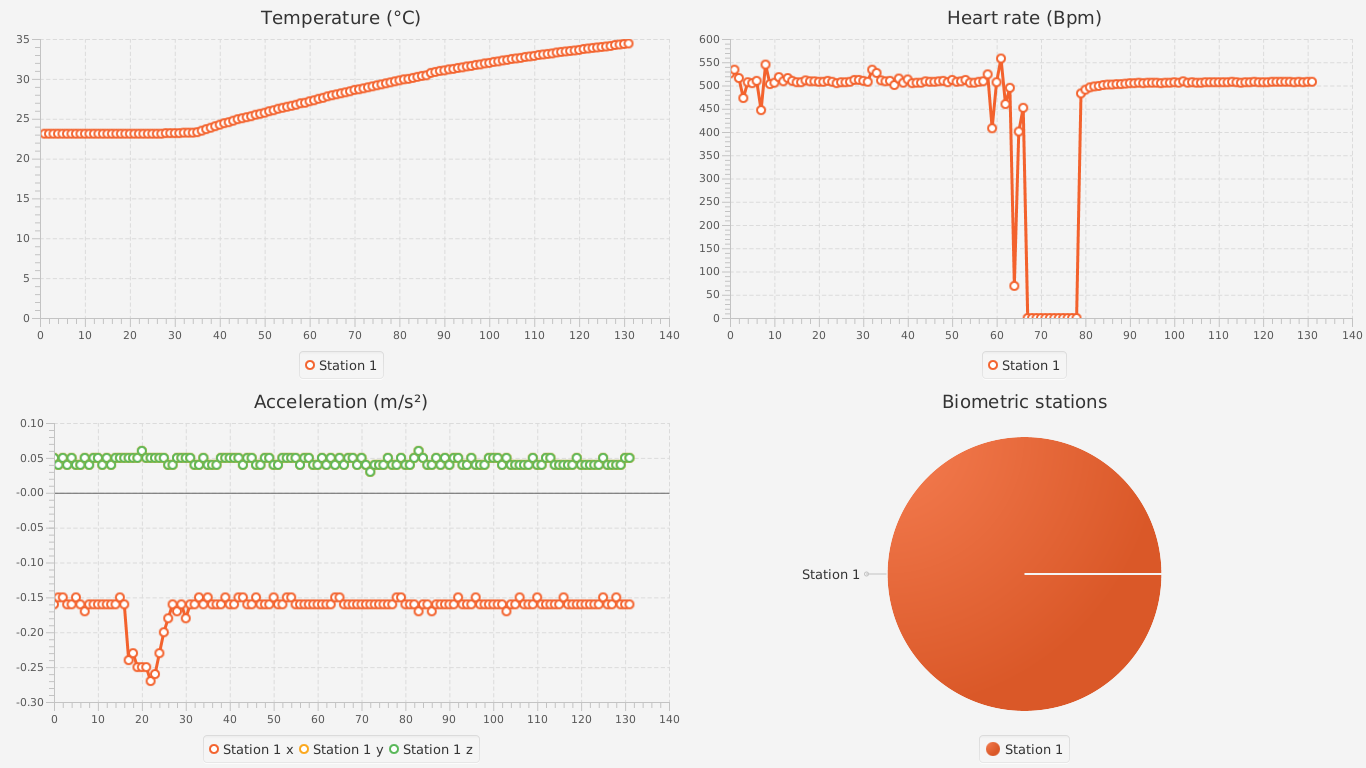
\includegraphics[width=\textwidth]{gui}\\
    Dit is een screenshot van de temperatuursensor die opwarmt.
    Zie ook de video \code{Testing.mkv} om een voorbeeld te zien van de volledige werking.

\chapter{Besluiten}

\begin{thebibliography}{9}
    \bibitem{accel1} \textit{Accelerometer}, SM, 2015/07/28, \url{https://www.arduino.cc/en/Tutorial/ADXL3xx}.
    \bibitem{accel2} \textit{Accelerometer}, Jonathanrjpereira, 2016/02/10, \url{http://www.instructables.com/id/Ultimate-Guide-to-Adruino-Serial-Plotter/}.
    \bibitem{accel3} \textit{Accelerometer}, JIMB0, 2014/06/11, \url{https://learn.sparkfun.com/tutorials/mma8452q-accelerometer-breakout-hookup-guide/all}.
    \bibitem{accel4} \textit{Accelerometer}, Louis Moreau, 2018/02/23, \url{https://github.com/sigfox-earthquake/Arduino-MKRFox-MMA8452/blob/master/Arduino-MKRFox-MMA8452.ino}.
    \bibitem{accel5} \textit{Accelerometer}, ToniCorinne, 2015/05/14, \url{https://github.com/sparkfun/SparkFun_MMA8452Q_Arduino_Library/tree/V_1.1.0}.
    
    \bibitem{heart1} \textit{Hartslagsensor}, SM, 2015/07/29, \url{https://www.arduino.cc/en/Tutorial/Graph}.
    \bibitem{heart2} \textit{Hartslagsensor}, MobiusHorizons, 2017/04/02, \url{https://www.youtube.com/watch?v=BPHinoRZOK4}.
    \bibitem{heart3} \textit{Hartslagsensor}, Pulse Sensor, 2017/03/23, \url{https://www.youtube.com/watch?v=82T_zBZQkOE}.
    \bibitem{heart4} \textit{Hartslagsensor}, VE7JRO, 2017/08/23, \url{https://arduino.stackexchange.com/questions/43956/getting-bpm-from-the-given-code}.
    \bibitem{heart5} \textit{Hartslagsensor}, yury-g, 2017/01/26, \url{https://github.com/WorldFamousElectronics/PulseSensor_Amped_Arduino/blob/master/PulseSensorAmped_Arduino_1.5.0/PulseSensorAmped_Arduino_1.5.0.ino}.
    \bibitem{heart6} \textit{Hartslagsensor}, biomurph, 2018/02/27, \url{https://pulsesensor.com/pages/getting-advanced}.
    \bibitem{heart7} \textit{Hartslagsensor}, Joel Murphy, Yury Gitman, lente van 2013, \url{http://www.theorycircuit.com/pulse-sensor-arduino/}.
    
    \bibitem{temp1} \textit{Temperatuursensor}, ALEX THE GIANT, 2017/02/02, \url{https://learn.sparkfun.com/tutorials/tmp102-digital-temperature-sensor-hookup-guide}.
    \bibitem{temp2} \textit{Temperatuursensor}, Texas Instruments, 2017/10/31, \url{https://www.youtube.com/watch?v=G0Gn3oQTLaI}.
    \bibitem{temp3} \textit{Temperatuursensor}, awende, 2016/08/15, \url{https://github.com/sparkfun/SparkFun_TMP102_Arduino_Library/blob/master/examples/SparkFun_TMP102_Breakout_Example/SparkFun_TMP102_Breakout_Example.ino}.
                    
    \bibitem{lcd1} \textit{LCD, 2017/04/14}, \url{http://linksprite.com/wiki/index.php5?title=16_X_2_LCD_Keypad_Shield_for_Arduino_V2}.
    \bibitem{lcd2} \textit{LCD, David Riewe}, 2015/12/30, \url{http://hackerspacetech.com/lcd-button-shield-v2-for-arduino-by-sparkfun.html#.WvRSWoiFNPZ}.
\end{thebibliography}
    
\end{document}
